\section{Introduction}
\label{sect:introduction}

\subsection{What is a mesh?}
\label{ssect:mesh_definition}
\par
A mesh can be qualitatively thought of as the tessellation of a domain $\Omega$ into a set of
non-overlapping subdomains $\omega_i$:
\begin{align}
\Omega &= \cup \left\{ \omega_i \left| i=1,2,\ldots ele \right. \right\} \nonumber \\
\label{eqn:tessalation_definition} \\
0 &= \cap \left\{ \omega_i \left| i=1,2,\ldots ele \right. \right\} \nonumber
\end{align}
where $ele$ is the number of elements in the tessellation. Figure \ref{fig:1d_2d_mesh_examples} shows
meshes on one-dimensional and two-dimensional domains. The extension to three-dimensional domains
is clear. Whatever the dimensionality of the domain, it is evident from figure \ref{fig:1d_2d_mesh_examples} that the mesh can be constructed
by first distributing a set of nodes throughout the domain, and then connect the nodes, so as to obtain
a set of non--overlapping elements. Therefore, in order to define a mesh, one needs to define node locations,
as well as element topology consistent to equations \eqref{eqn:tessalation_definition}.
\begin{figure}[htbp]
 \centering
  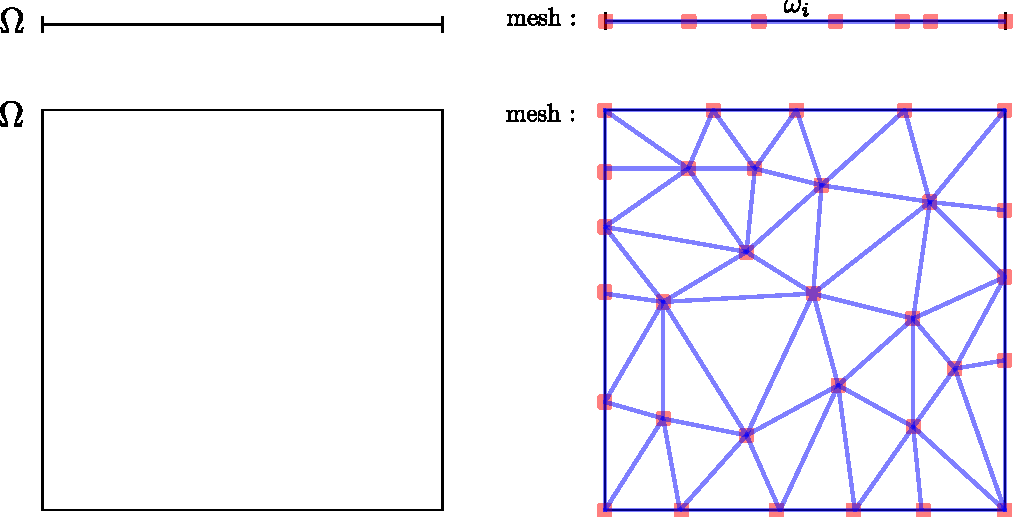
\includegraphics[width=1.0\textwidth]{../figures/1d_2d_mesh_examples}
  \caption{Examples of meshes in one-dimensional and two-dimensional domains.}
  \label{fig:1d_2d_mesh_examples}
\end{figure}

\subsection{What is Gmsh?}
\label{sect:Gmsh}
\par
It is the task of a \emph{mesh generator} to create node locations and element topology so as to create high quality meshes. Gmsh is a \emph{``3D finite element grid generator with a build-in CAD engine and post-processor. Its design goal is to provide a fast, light and user-friendly meshing tool with parametric input and advanced visualisation capabilities.''}\footnote{from \url{http://www.geuz.org/gmsh/}}. Furthermore, Gmsh can be used as a 1--, 2-- and 3-- dimensional mesh generator for use with Fluidity.
\par
Gmsh is developed by~\cite{Geuzaine_Remacle_2009} and distributed under the terms of the GNU General Public License. Executables for Linux, Windows and Mac OS can be downloaded from \url{http://www.geuz.org/gmsh/} as well as the source code. In Linux distributions where the Advanced Package Tool (APT) is available (such as Ubuntu), typing \lstinline{sudo apt-get install gmsh} in a terminal will probably install Gmsh on your system. The rest of this tutorial assumes that Gmsh is run on Linux. 
\par
Gmsh's architecture is centred around four modules:
\begin{enumerate}
  \item Geometry
  \item Mesh
  \item Solver
  \item Post-processing
\end{enumerate}
In this tutorial we will only use the Geometry and Mesh modules. As suggested by their names the geometry
module is used to define geometrical objects, such as points, lines, surfaces and volumes, while the
mesh module is used to create meshes (nodes and element topology).

\subsubsection{Starting Gmsh}
\begin{figure}[htbp]
 \centering
  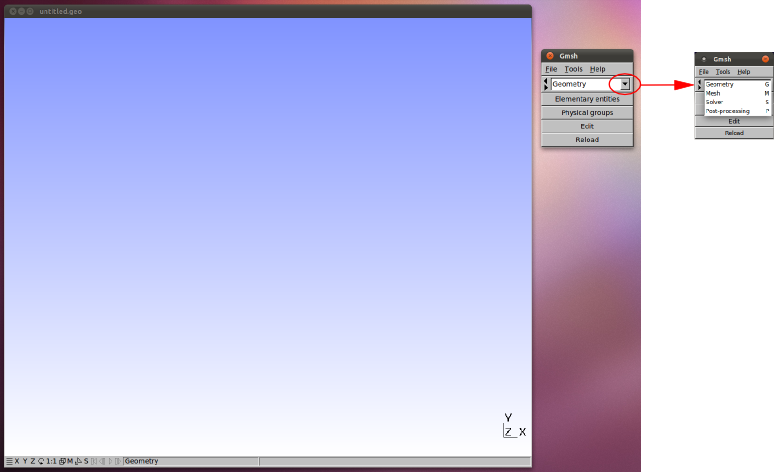
\includegraphics[width=1.0\textwidth]{../figures/gmsh_startup_and_modules.png}
  \caption{Left panel: The Gmsh windows after startup. The larger window is termed the Graphic window
           and the smaller window is termed the Menu window.}
  \label{fig:gmsh_startup_and_modules}
\end{figure}
Gmsh can be started by issuing the following command at the Terminal:
\begin{lstlisting}
gmsh mymesh.geo
\end{lstlisting}
where \lstinline{mymesh.geo} is the name of the newly created file to store your geometry. If a file is
not named, an \lstinline{untitled.geo} file will be created. For this tutorial, it is best practice to
name your files and avoid using an ``untitled'' document. As the Gmsh user interacts with the GUI,
her/his actions are stored in the \lstinline{.geo} file, in the form of script commands. One can modify
the script with any text editor. Once Gmsh is opened, you will be presented with the Gmsh
\emph{menu} and \emph{graphic} windows, as illustrated in
figure~\ref{fig:gmsh_startup_and_modules}.

\subsubsection{Basic interaction with the Graphical User Interface}
\label{ssect:basic_interaction_gmsh_gui}

Once Gmsh is opened, you will be presented with the Gmsh \emph{menu} and \emph{graphic} windows, as
illustrated in figure~\ref{fig:gmsh_startup_and_modules}.
The \emph{menu window} allows the user to access features of the Gmsh graphical user interface, while
the \emph{graphic window} displays the defined points, lines and any other geometrical objects. The
modular architecture of Gmsh is reflected in the menu window; clicking on the down-pointing arrow next
to ``Geometry'' produces a drop-down menu (as shown in figure \ref{fig:gmsh_startup_and_modules}),
allowing the user to select any of the four modules listed in section \ref{sect:Gmsh}.
\begin{figure}[htbp!]
 \centering
  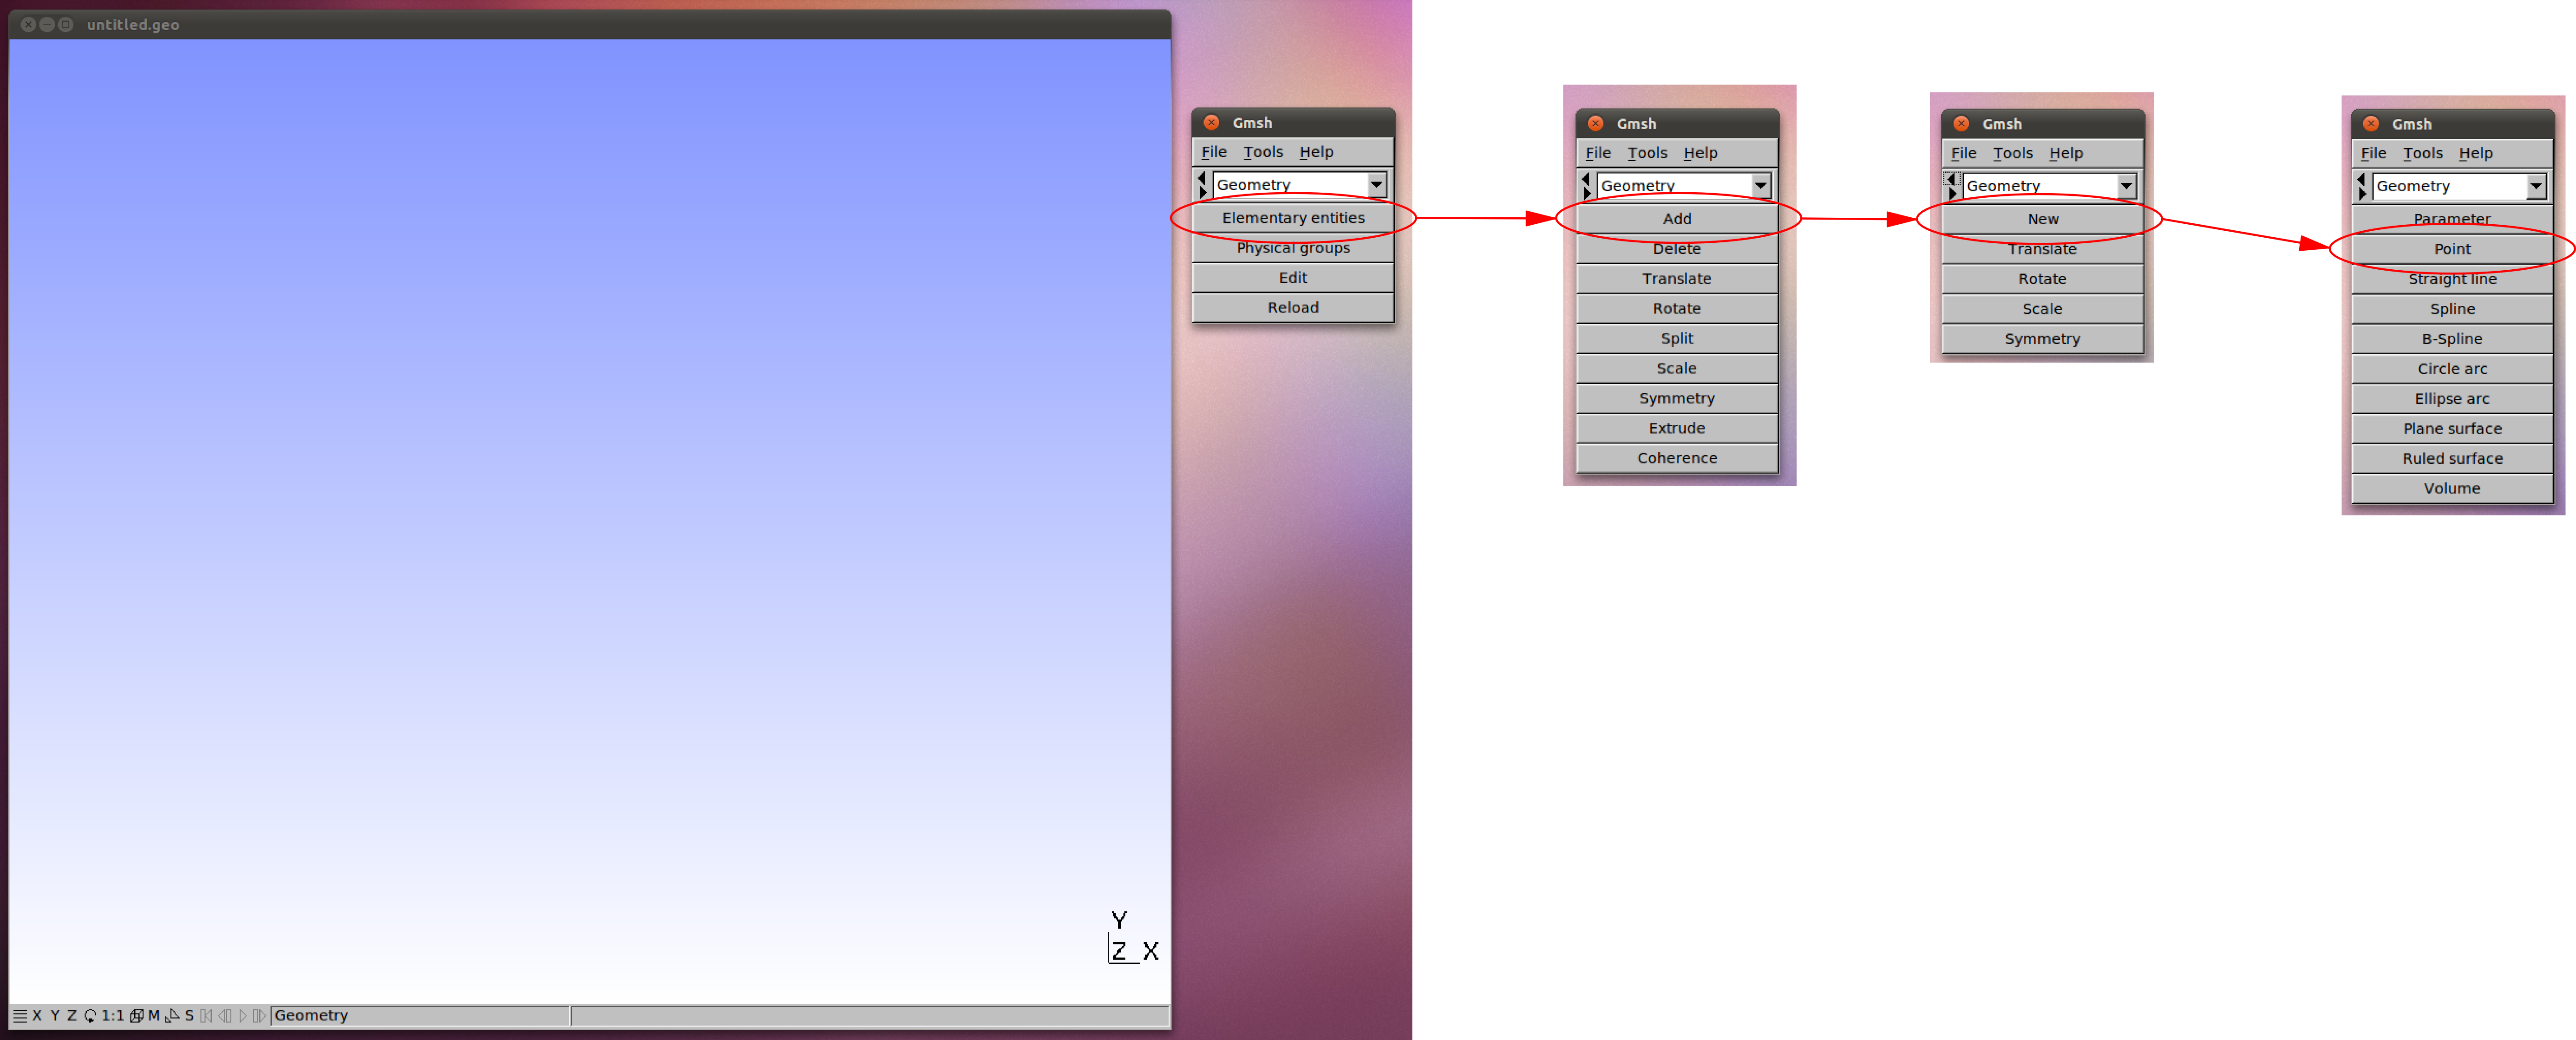
\includegraphics[width=1.0\textwidth]{../figures/getting_started.png}
  \caption{Basic interaction with the GMSH GUI}
  \label{fig:basic_interaction}
\end{figure}
Familiarise yourself with the Gmsh menu window, by navigating to a mode that allows you to add a point.
Try the following for yourself to get comfortable navigating the menu and understand the notation
provided above, which will be used through this tutorial to point you to specific features of Gmsh.
\begin{enumerate}
  \item Click on \lstinline{Geometry (G) > Elementary entities > Add > New > Point}, as indicated in
        figure \ref{fig:basic_interaction}. After clicking on ``Point'' in the menu window the 
        ``Contextual Geometry Definitions'' window will appear and a message appears at the top
        of the Graphic window, as shown in figure \ref{fig:creating_a_point}.
  \item Close the Contextual Geometry Definitions window and press ``q'' to abort the command.
  \item You may use the keyboard buttons $G$, $M$, $S$ and $P$ to get to the top-level of the
        Geometry, Mesh, Solvers and Post-processing modules respectively. Press $G$ to return to
        the top-level of the Geometry module. Try switching to the Mesh module and then back to
        the Geometry module.
\end{enumerate}

\begin{figure}[htbp]
 \centering
  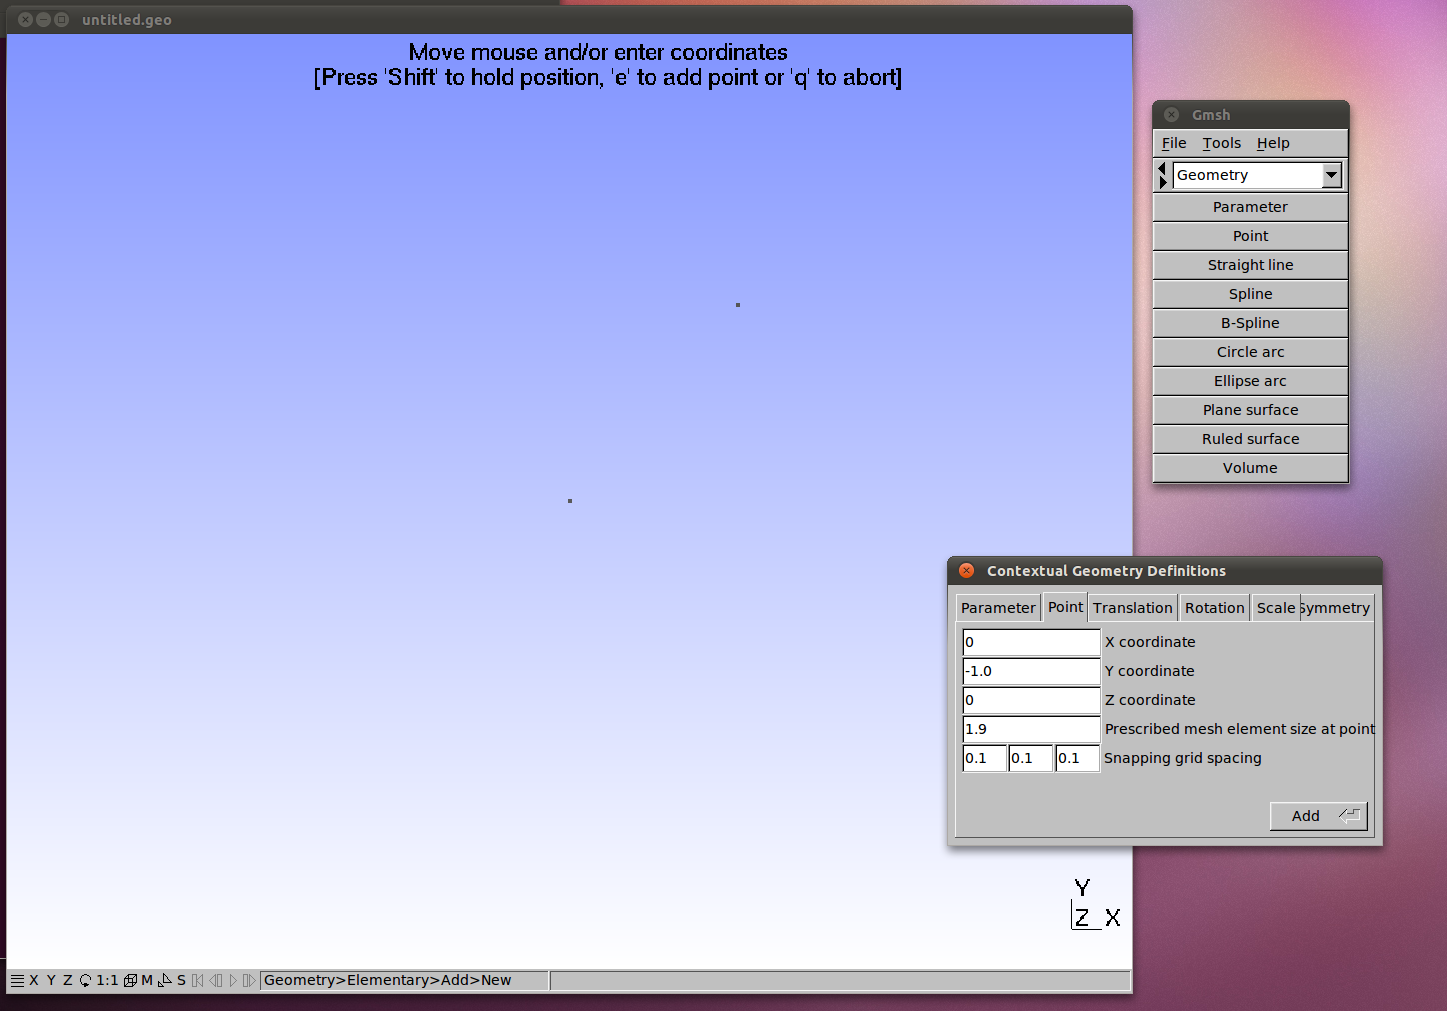
\includegraphics[width=0.8\textwidth]{../figures/shot5.png}
  \caption{Creating a point.}
  \label{fig:creating_a_point}
\end{figure}

We will now open an existing geometry and learn to navigate by panning, zooming and rotating. To obtain the geometry, please download the file at:
\begin{lstlisting}
http://amcg.ese.ic.ac.uk/download/annulus.geo
\end{lstlisting}
and open it by issuing the following at the command line:
\begin{lstlisting}
gmsh annulus.geo
\end{lstlisting}

Once open, you should see the geometry illustrated in figure~\ref{fig:annulus1}. On the bottom-left of the graphic window,
you will see various tools available to manage the view.
The $X$, $Y$ and $Z$ buttons align the corresponding axis perpendicular to the screen. Try selecting the
$X$ view, as in figure~\ref{fig:annulus2}. Both these views are not particularly useful in understanding
the annulus domain. Try to rotate the geometry by left-clicking and holding on the screen, then moving the mouse pointer.
Try to get the geometry as illustrated in figure~\ref{fig:annulus3}. You can pan the geometry by right-clicking and moving the mouse. To zoom, simply use the scroll. Alternatively, you may hold the middle-button and move the mouse. Make sure you familiarise yourself with manipulating the orientation of your domain, as this will be useful later on.

\begin{figure}[htbp!]
  \centering
  \subfloat[Default view]{\label{fig:annulus1}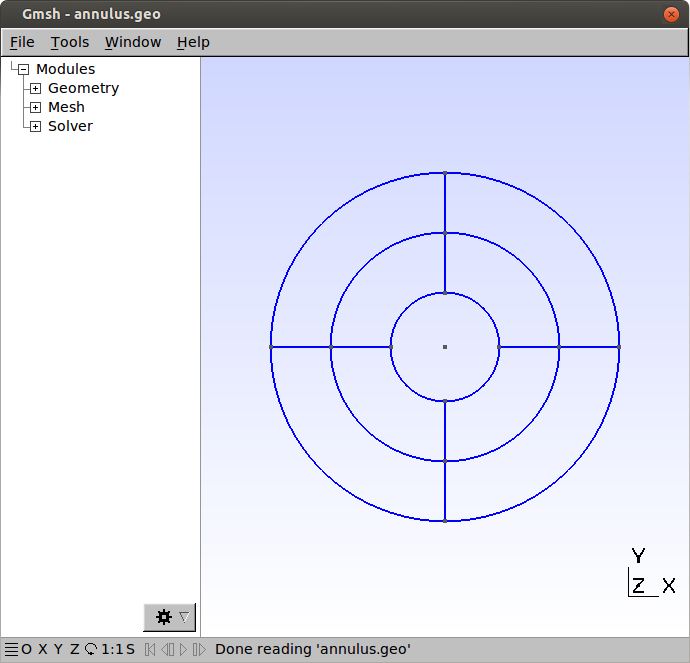
\includegraphics[width=0.45\textwidth]{../figures/annulus1}}
  \subfloat[x--axis perpendicular to screen]{\label{fig:annulus2}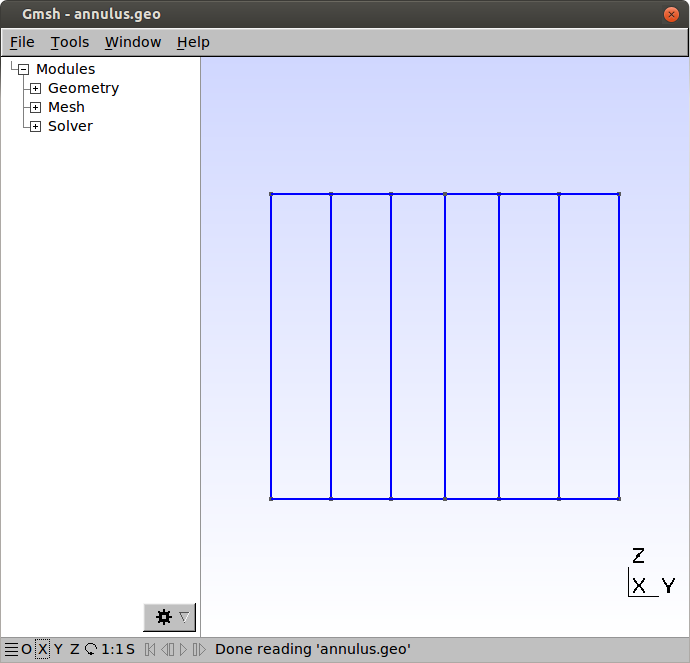
\includegraphics[width=0.45\textwidth]{../figures/annulus2}}\\
  \subfloat[Rotated view]{\label{fig:annulus3}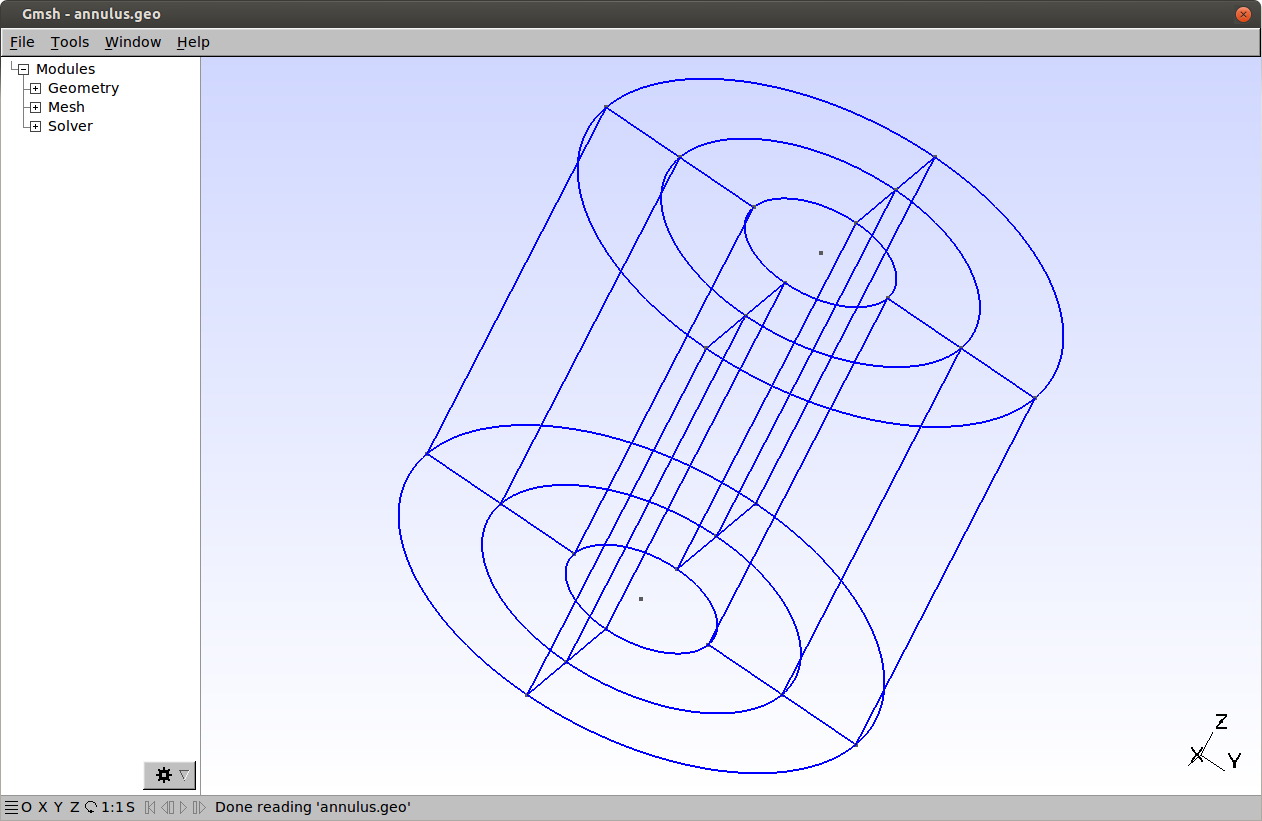
\includegraphics[width=0.45\textwidth]{../figures/annulus3}}
  \subfloat[Meshed and zoomed]{\label{fig:annulus4}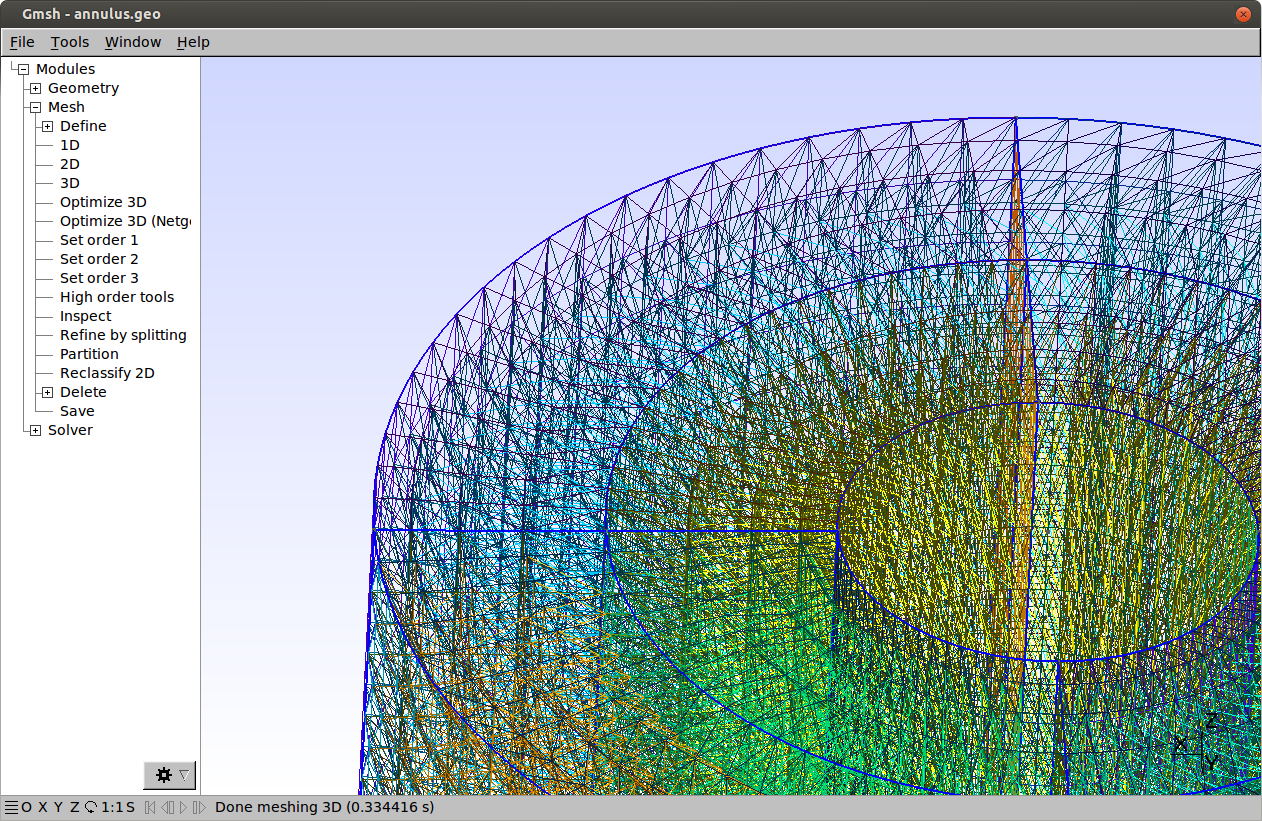
\includegraphics[width=0.45\textwidth]{../figures/annulus4}}
  \caption{Panning, zooming, rotating and manipulating the Gmsh graphic window.}
  \label{fig:animals}
\end{figure}
\par
As no meshing tutorial can be complete without a mesh, we end by meshing the geometry. To generate a mesh of this domain, go to:
\begin{lstlisting}
Mesh (M) > 3D
\end{lstlisting}
This can be done by pressing your keyboard's $M$ key, and then selecting $3D$ to mesh the three--dimensional domain. Figure \ref{fig:annulus4} shows a view of the meshed annulus.

